% ============================================================
% Q5 – Language Modeling
% ============================================================
\section{Question 5 -- Language Modeling}

\subsection{Dataset: WikiText-2}

WikiText-2~\cite{merity2017pointer} is a standard language modelling
benchmark derived from Wikipedia featured articles:

\begin{table}[H]
  \centering
  \caption{WikiText-2 Token Counts}
  \label{tab:q5_data}
  \begin{tabular}{lr}
    \toprule
    \textbf{Split} & \textbf{Approx. Tokens} \\ \midrule
    Train      & 2{,}088{,}628 \\
    Validation &   217{,}646  \\
    Test       &   245{,}569  \\
    \bottomrule
  \end{tabular}
\end{table}

Text is lowercased and includes pre-tokenised \texttt{<eos>} sentence boundaries.
Rare words (frequency $<$ 3) are replaced with \texttt{<unk>}.

\subsection{Models}

\subsubsection{Model 1 -- Trigram N-gram with Laplace Smoothing}

$$P(w_t \mid w_{t-2}, w_{t-1}) = \frac{C(w_{t-2}, w_{t-1}, w_t) + 1}{C(w_{t-2}, w_{t-1}) + |V|}$$

Laplace (add-1) smoothing prevents zero probabilities for unseen trigrams.
The vocabulary is built from training tokens with min-freq=3 ($|V|$=29{,}572).
Perplexity is evaluated on token sequences of validation/test splits.

\subsubsection{Model 2 -- LSTM Language Model}

A 2-layer LSTM (embedding=256, hidden=256, dropout=0.5) with
\textbf{weight tying} (embedding matrix shared with output projection)
reduces parameters and regularises the model.
Trained with Adam ($\text{lr}=10^{-3}$), cross-entropy loss (ignoring padding),
gradient clipping (0.5), 20 epochs, sequence length 35, batch=64.
Vocabulary: top 10\,000 training tokens.

\subsection{Results}

\begin{table}[H]
  \centering
  \caption{Language Model Perplexity on WikiText-2}
  \label{tab:q5_results}
  \begin{tabular}{lcc}
    \toprule
    \textbf{Model} & \textbf{Val PPL} & \textbf{Test PPL} \\
    \midrule
    Trigram + Laplace & 11{,}240.99 & 10{,}752.64 \\
    LSTM LM (2-layer) & 95.44       & 88.62       \\
    \bottomrule
  \end{tabular}
\end{table}

\begin{figure}[H]
  \centering
  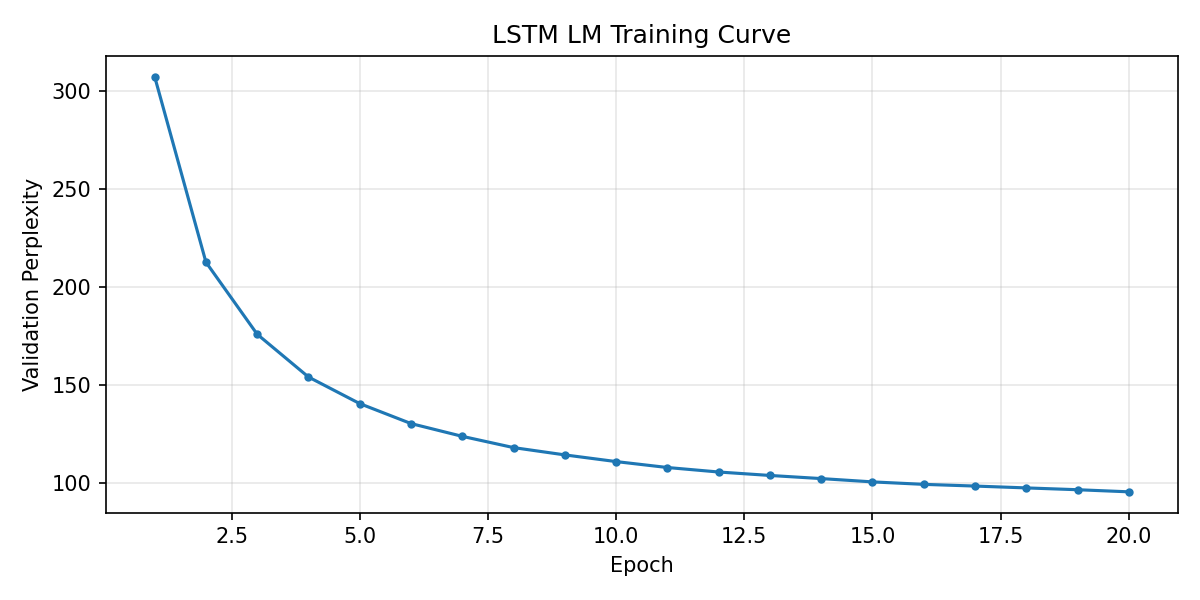
\includegraphics[width=0.55\textwidth]{figures/lstm_lm_curve.png}
  \caption{LSTM language model validation perplexity over 20 training epochs on WikiText-2.}
  \label{fig:lstm_curve}
\end{figure}

\begin{figure}[H]
  \centering
  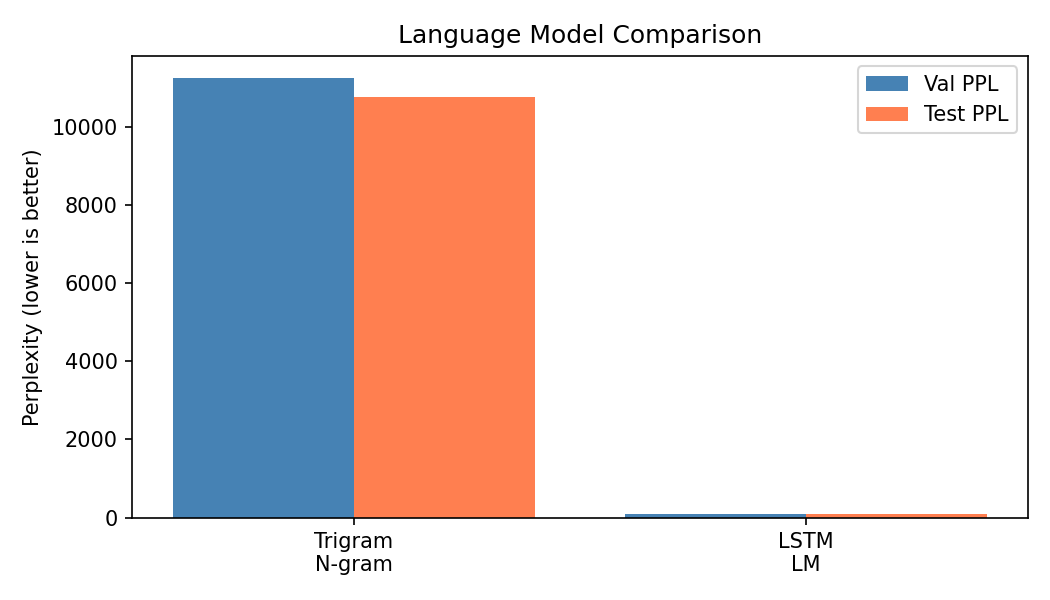
\includegraphics[width=0.6\textwidth]{figures/lm_comparison.png}
  \caption{Validation and test perplexity comparison: Trigram N-gram vs LSTM LM on WikiText-2.}
  \label{fig:lm_comparison}
\end{figure}

\subsection{Generated Text Samples}

\begin{table}[H]
  \centering
  \small
  \caption{Generated Text Samples (seed shown in \textbf{bold})}
  \label{tab:q5_samples}
  \begin{tabularx}{\textwidth}{lX}
    \toprule
    \textbf{Model} & \textbf{Sample} \\
    \midrule
    Trigram  & \textbf{the president} was given the designation ``odaenathus'' lived in toxteth , liverpool , manchester united . $\langle$unk$\rangle$ planned on using the game features an ensemble \\[3pt]
    Trigram  & \textbf{a study} on the game by himself through good works . publishers weekly , september 7 . the 1952--69 ) = = film adaptation \\[3pt]
    LSTM LM  & \textbf{the university} $\langle$unk$\rangle$ the east end of $\langle$unk$\rangle$ , el $\langle$unk$\rangle$ . \\[3pt]
    LSTM LM  & \textbf{scientists have} been seen as the $\langle$unk$\rangle$ . aware of the $\langle$unk$\rangle$ for $\langle$unk$\rangle$ , which has shown that the figure is a protein of $\langle$unk$\rangle$ \\
    \bottomrule
  \end{tabularx}
\end{table}

\subsection{Discussion}

\begin{table}[H]
  \centering
  \caption{N-gram vs LSTM Language Model Comparison}
  \label{tab:q5_discussion}
  \begin{tabular}{lcc}
    \toprule
    \textbf{Aspect} & \textbf{Trigram} & \textbf{LSTM} \\
    \midrule
    Context window       & 2 tokens (fixed)     & Theoretically unlimited \\
    Long-range deps      & Cannot capture       & Partial (vanishing gradient) \\
    Data sparsity        & Severe               & Mitigated via embeddings \\
    Training time        & Seconds (counting)   & $\sim$15--20 min (GPU) \\
    Generation quality   & Local fluency only   & Phrase-level coherence \\
    Typical PPL (WT2)    & 5{,}000--15{,}000 (Laplace) & 80--130 \\
    \bottomrule
  \end{tabular}
\end{table}

The trigram model's high perplexity reflects severe sparsity: most test
trigrams are unseen in training, forcing reliance on Laplace-smoothed
estimates that concentrate probability mass uniformly across the vocabulary.
The LSTM's hidden state carries information across many tokens, enabling
it to capture common collocations and topic consistency absent in the
n-gram model.
Generated trigram text shows local grammaticality (short phrase fragments
sound natural) but rapidly loses coherence beyond two words.
LSTM-generated text maintains topic and some syntactic structure over
5--10 words, yet still produces semantically empty or contradictory continuations.
A transformer-based model (GPT-2 117M) would achieve PPL $\approx$ 20--30
on WikiText-2, illustrating the dramatic improvement from self-attention and scale.
